\textbf{3. MATLAB fun.} Digitally generate a large number of random probability density functions. An example might be\\
\begin{center}
  \texttt{    S=rand(N,1);}  \\
  \texttt{    fX=S/sum(S);} \\
\end{center}
The value or $N$ can vary for each density.
\begin{enumerate}[(a)]
\item  Evaluate the mean and variance of each density.\\
  \textbf{Solution:}\\
  Code segment used is shown in listing~\ref{lst:p3a}, result is shown in figure~\ref{fig:p3a}
  \CodeSnippet{matlab}{Code used to generate all the pics}{lst:p3a}{../src/matlab/problem3.m}{1}{48}
  \begin{figure}[!h]
    \begin{center}
      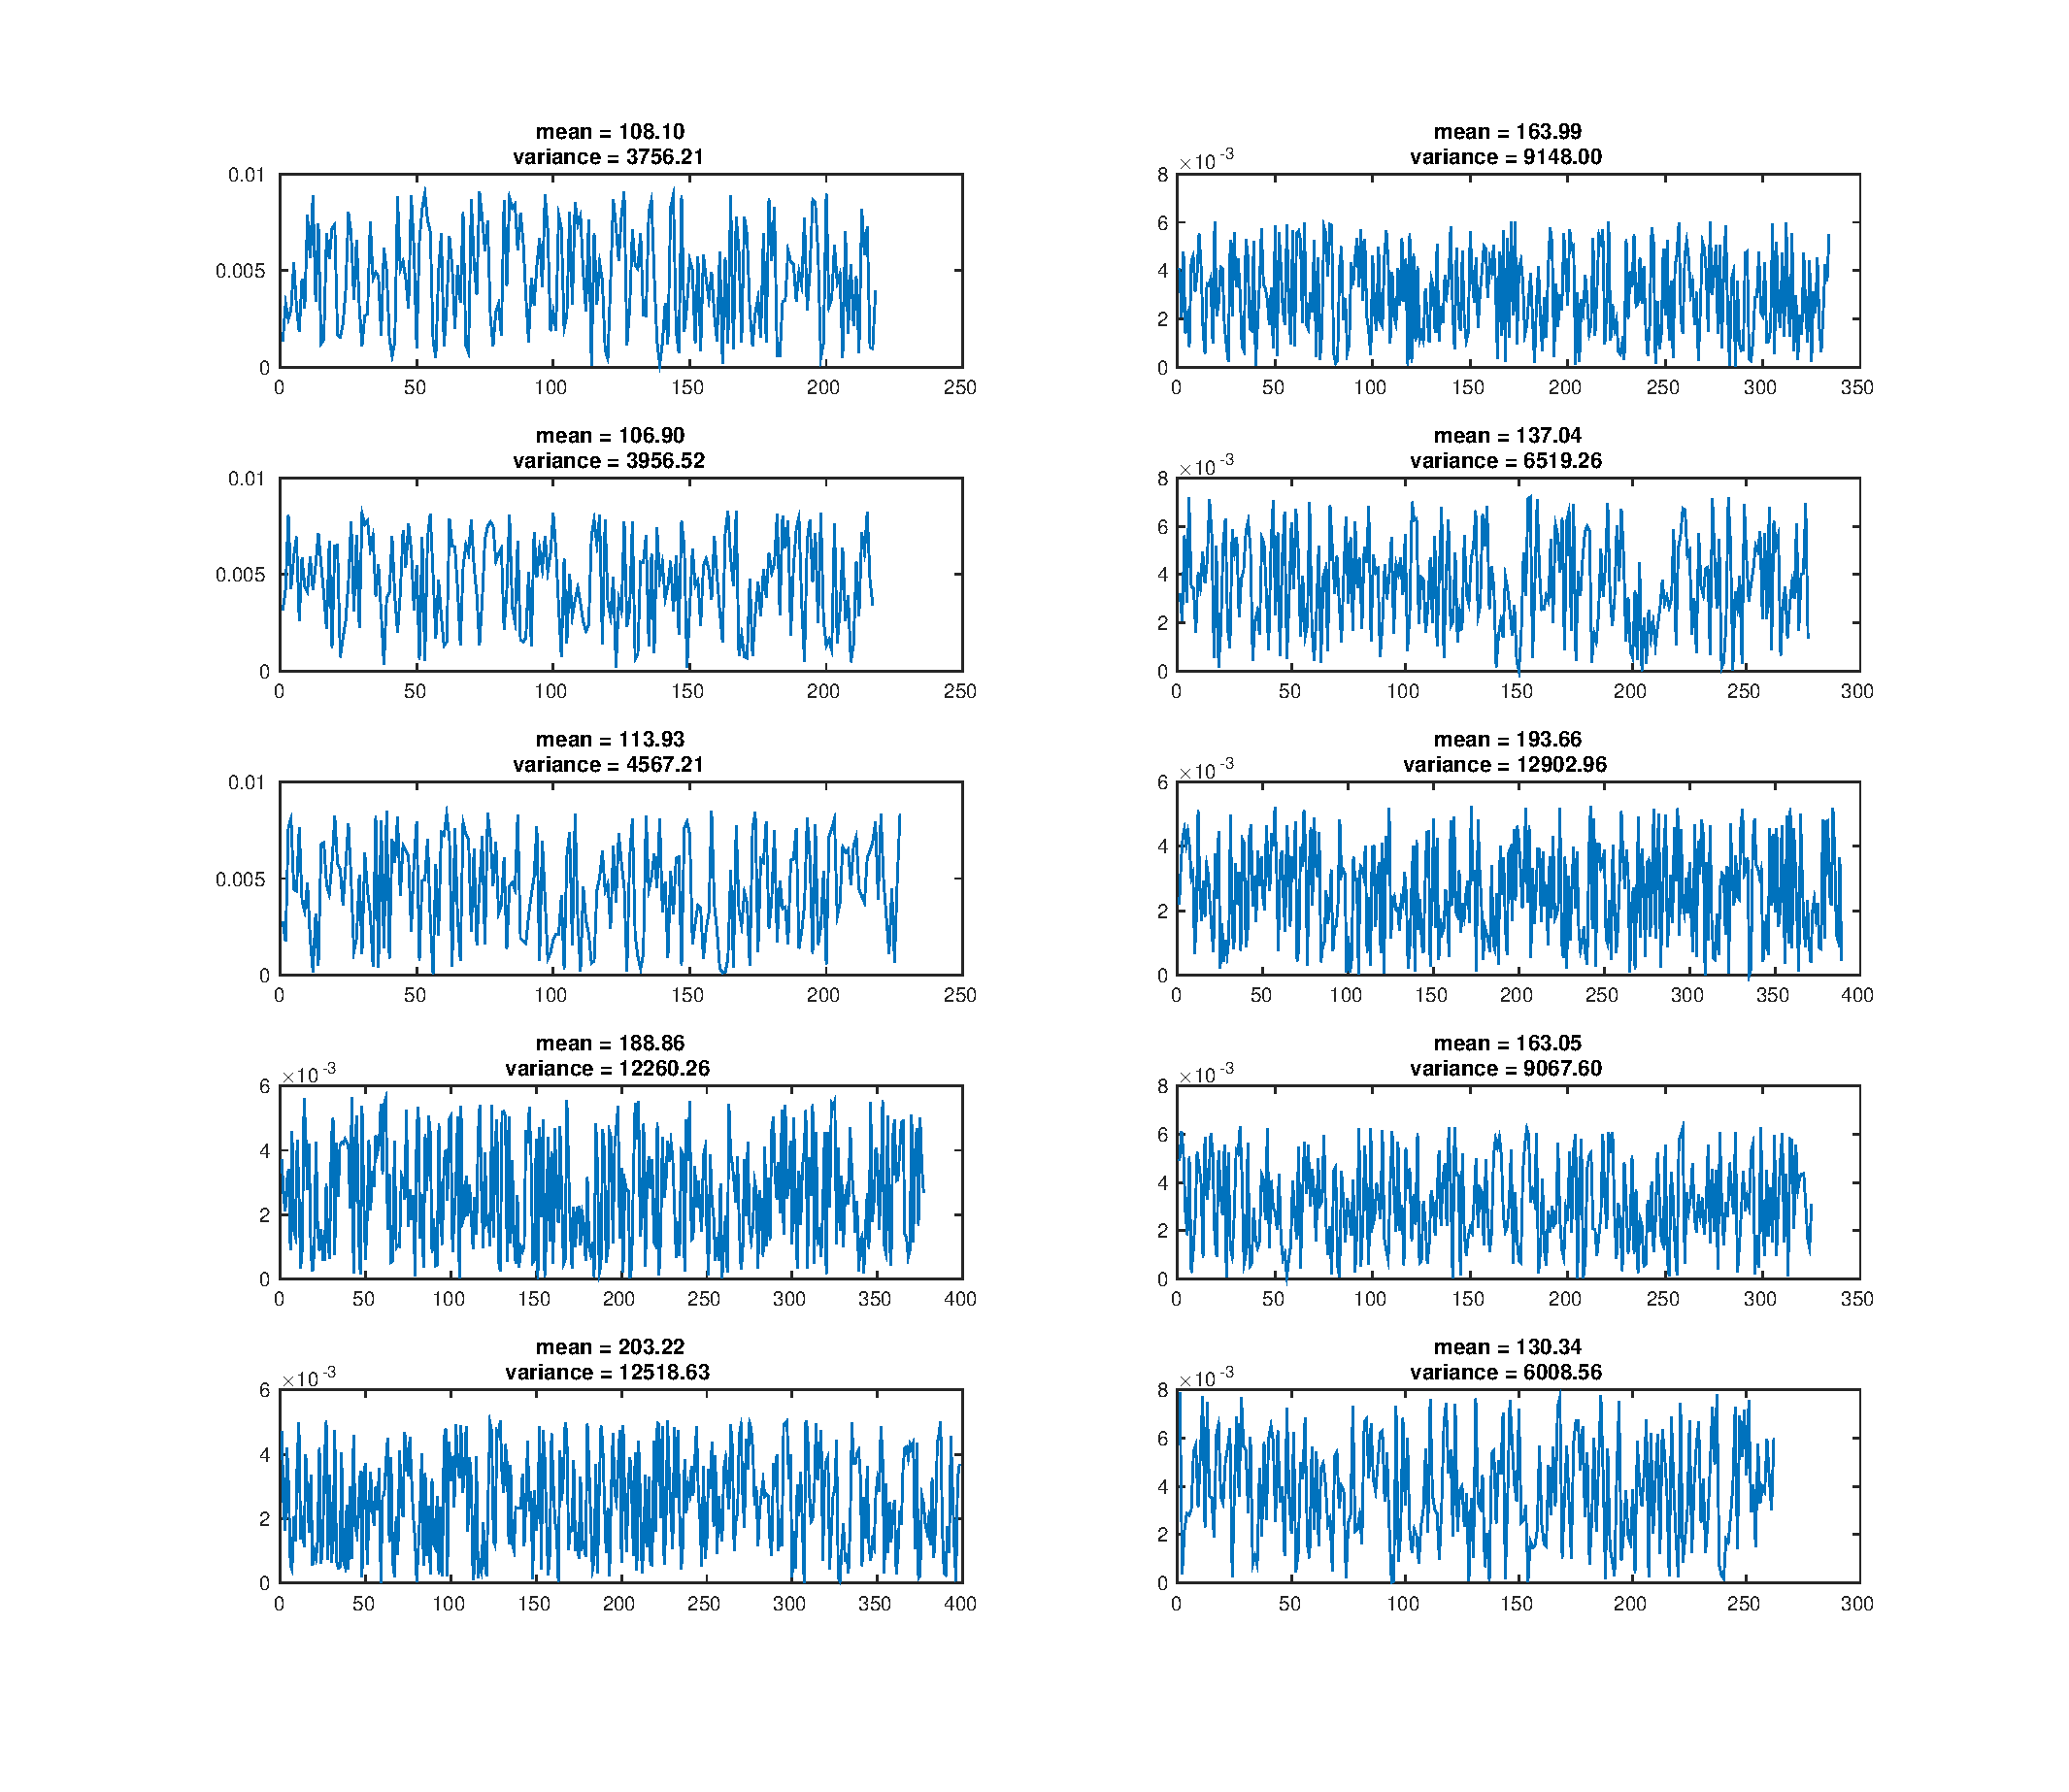
\includegraphics[width=6in]{random_distributions.eps}
    \end{center}
    \caption{Generated random distributions with their means and variances calculated.}
    \label{fig:p3a}
  \end{figure}

\item  Convolve the densities. There is a MATLAB function called \\
  \begin{center}
    \texttt{    conv;}    \\
  \end{center}
  Code segment contuned from part (a) is shown in listing~\ref{lst:p3b}
  \CodeSnippet{matlab}{Convolve all the distributions}{lst:p3b}{../src/matlab/problem3.m}{49}{70}

\item  Calculate the mean and variance of the convolution and verify the mean is the sum of the means and the variance is the sum of the variances.
  \CodeSnippet{matlab}{Code used to generate all the pics}{lst:problem3}{../src/matlab/problem3.m}{71}{79}

  outputs:
  \color{lightgray}
\begin{verbatim}
difference of mean     : 9.00
difference of variance : 0.00
\end{verbatim}
  \color{black}

\item  On the same graph, plot the convolution and the Gaussian approximation using the
  central limit theorem.
  \CodeSnippet{Matlab}{Code used to generate all the pics}{lst:problem3}{../src/matlab/problem3.m}{80}{86}
  \begin{figure}[!h]
    \begin{center}
      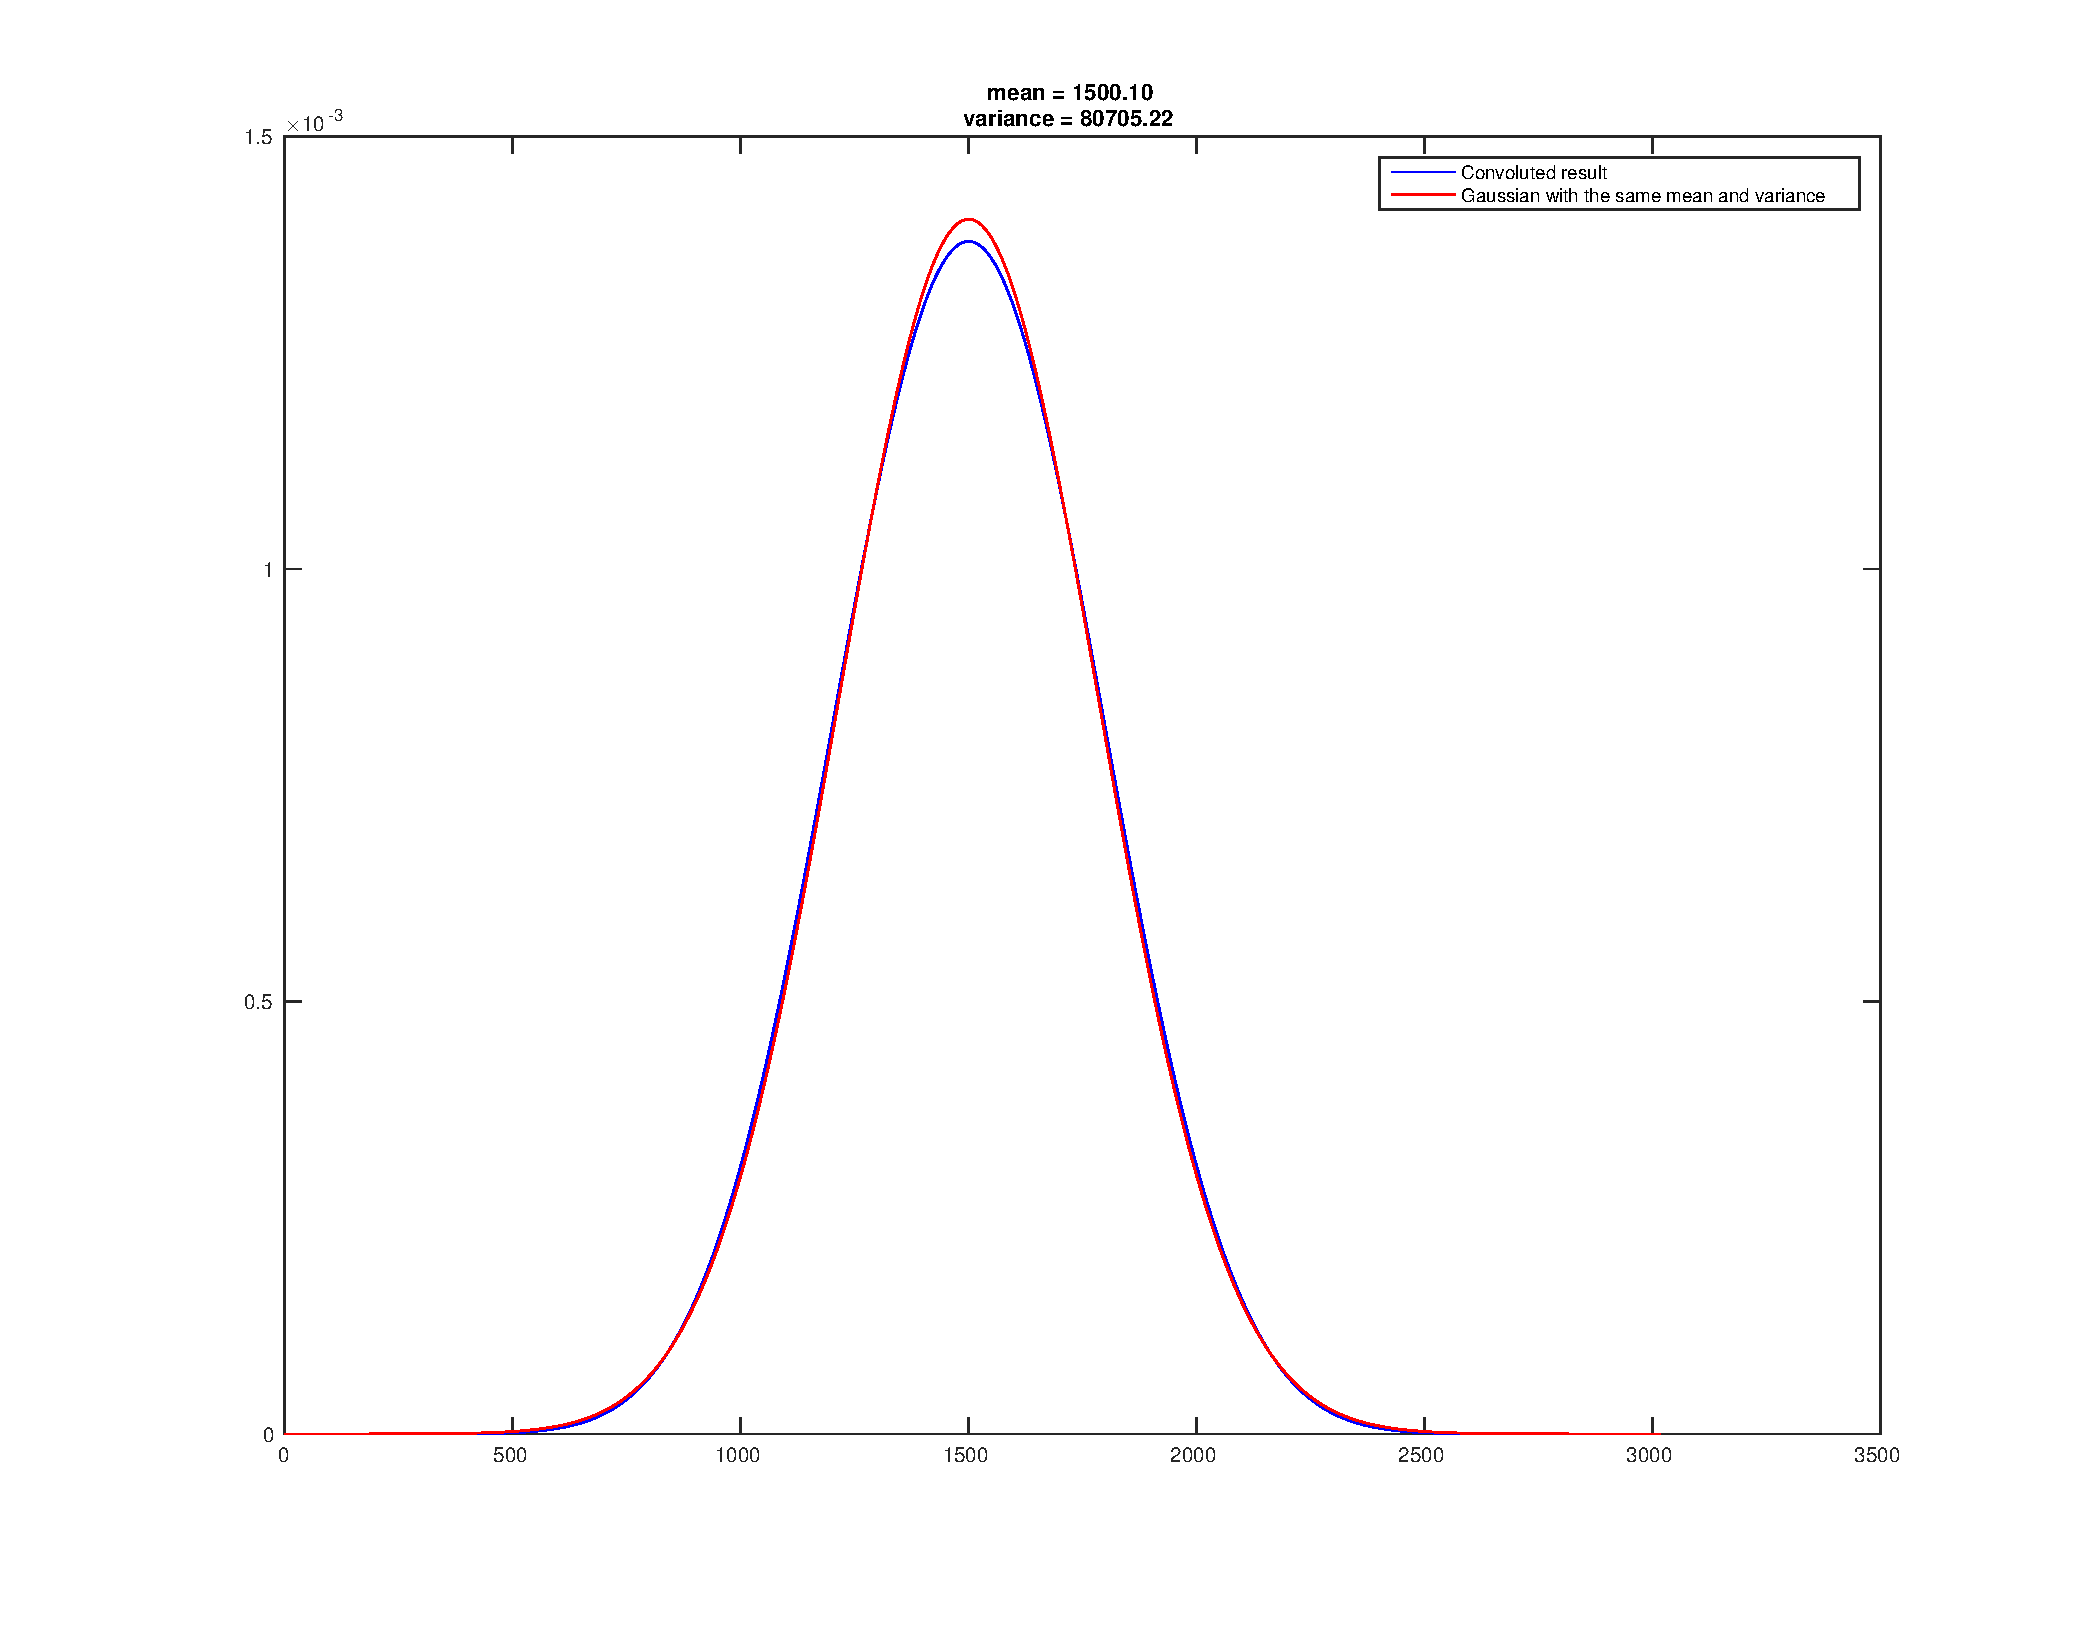
\includegraphics[width=6in]{gaussian.eps}
    \end{center}
      \caption{Convoluted distribution and gaussian pdf withe the same mean and variance}
      \label{fig:conv_gauss}
  \end{figure}
\end{enumerate}



